\documentclass[11pt]{article}
\usepackage[margin=3cm]{geometry}
\usepackage[swedish]{babel}
\usepackage[utf8]{inputenc}
\usepackage[T1]{fontenc}
\usepackage{fancyhdr}
\usepackage{ragged2e}
\usepackage{titling}
\usepackage{graphicx}
\usepackage{pbox}
\usepackage{tabularx}
\usepackage{longtable}
\usepackage{tabu}
\usepackage{url}
\usepackage{float}
\usepackage[hidelinks]{hyperref}
\usepackage[backend=biber,style=ieee]{biblatex}
\usepackage{csquotes}

\addbibresource{refs.bib}
\graphicspath{ {images/} }
\newcommand{\subtitle}[1]{%
  \posttitle{%
    \par\end{center}
    \begin{center}\large#1\end{center}
    \vskip0.5em}%
}


\newcounter{refc}
\setcounter{refc}{1}
\newcommand{\reff}{
	\therefc
	\stepcounter{refc}
}

\pagestyle{fancy}


\date{}
\pagenumbering{roman}
\chead{Förstudie - Sensorer}
\rhead{\today}
\lhead{}
\lfoot{
	TSEA56 
	\\
	ISY
}
\rfoot{
	Andreas Brorsson \textit{Andbr981}
	\\
	Nikolaj Agafonov \textit{Nikag669}
}

\begin{document}
\begin{titlepage}
\begin{center}
TSEA56 - Kandidatprojekt i elektronik \\[0.5in]
{\Large\bfseries Förstudie - Sensorer }\\
%
\vspace{4\baselineskip}
%
Version 0.1\\
\vspace{2\baselineskip}
%
Grupp 2 \\
Agafonov, Nikolaj, 
\texttt{nikag669}
\\
Brorsson, Andreas, 
\texttt{andbr981}
\\


\vspace{2\baselineskip}
\today

\vspace{23\baselineskip}
Status
\begin{table}[b]
\centering
\begin{tabular}{|l|l|l|} \hline
 Granskad & -- & datum  \\ \hline
 Godkänd  & -- & datum \\ \hline 
\end{tabular}
\end{table}

\end{center}
\end{titlepage}

\pagebreak
\begin{center}

\section*{PROJEKTIDENTITET}
2015/VT, Undsättningsrobot Gr. 2
\\
Linköpings tekniska högskola, ISY
\\[0.5in]
\begin{table}[h]
\begin{tabular}{|l|p{0.3\linewidth}|l|l|} \hline
Namn & Ansvar & Telefon & E-post \\[0.1in] \hline
Nikolaj Agafonov & Dokumentansvarig (DA) & 072-276 99 46 & nikag669@student.liu.se \\ \hline
Adnan Berberovic & Projektledare (PL) & 070-491 96 07 & adnbe196@student.liu.se \\ \hline
Andreas Brorsson & Testansvarig (TA) & 073-524 44 60 & andbr981@student.liu.se \\ \hline
Fredrik Fridborn & Designansvarig Sensormodul (DSE) & 073-585 52 01 & frefr166@student.liu.se \\ \hline
Robert Oprea & Designansvarig Styrmodul (DST) & 070-022 10 18 & robop806@student.liu.se \\ \hline
Måns Skytt & Designansvarig Kommunikationsenhet (DK) & 070-354 28 84 & mansk700@student.liu.se \\ \hline
\end{tabular}
\end{table}


E-postlista för hela gruppen: adnbe196@student.liu.se
\\[1in]
Kund: Kent Palmkvist, 581 83 Linköping,
Kundtelefon: 013-28 13 47, kentp@isy.liu.se
\\
ISY-handledare: Kristoffer Öfjäll, kristoffer.ofjall@liu.se
\\
TEMA-handledare: Birgitte Saxstrup, birgitte.saxtrup@liu.se
\\[1in]
Kursansvarig: Tomas Svensson, 013-28 13 68, tomass@isy.liu.se
\\
Handledare: Olov Andersson, 013-28 26 58, Olov.Andersson@liu.se
\end{center}
\pagebreak

\tableofcontents

\pagebreak

\section*{Dokumenthistorik}
\begin{table}[h]
\begin{tabular}{|l|l|l|l|l|} \hline

Version & 
Datum & 
Utförda förändringar & 
Utförda av & 
Granskad \\[0.1in] \hline
0.1 &
2015-03-05 & 
Första utkastet & 
NA, ABr & 
\\ \hline

\end{tabular}
\end{table}


\pagebreak

\pagenumbering{arabic}

\begin{flushleft}

%% -------------------------------------- ////////// ---------------------

\section{Inledning}
Denna förstudie om sensorer tar upp frågeställningar som uppkommer när en autonom robot ska konstrueras. Vilka sensorer som kan passa till en undsättningsrobot och hur dessa fungerar. Vilken data de ger till roboten och i vilka storheter fås. Vad kan störa sensorerna och hur noggranna de är.

\subsection{Syfte}
Syftet med skrivuppgiften är att få möjlighet att individuellt träna och få återkoppling på tekniskt skrivande såväl innehållsmässigt som språkligt. 

\subsection{Mål}
Målet med förstudien är:
\begin{itemize}

\item Att introducera författarna till vetenskapligt och tekniskt skrivande och förbereda inför bland annat examensarbetet.

\item Att få en fördjupning i ämnet och en större kunskapsbas för sensorer.

\item Att resultatet ska komma fram till vilka sensorer som bör användas i byggandet av en undsättningsrobot i kursen TSEA56.

\end{itemize}
 
 
\subsection{Introduktion till Sensorer}
Sensorer är en anordning för att konvertera en form av energi till en annan form. Dessa energier kan vara elektromagnetiska, mekaniska eller akustiska till t ex en spänning. Då en dator behöver digital data för att kunna analysera sin omgivning kvantiseras spänningen från sensorn via en A/D-omvandlare till digital data som kan processeras. 
\\[0.1in]
Sensorer som den autonoma undsättningsroboten kan behöva är:
\begin{itemize}
\item Avståndssensorer för att mäta avståndet till väggar och hinder.

\item Reflektionssensor, för att få reda på när roboten har kommit fram till målet.

\item Gyro, för att läsa av hur mycket roboten har roterat vid svängar eller rotation.

\item RFID-avläsare.

\end{itemize}


\pagebreak

%% -------------------------------------- ////////// ---------------------

\section{Problemformulering}
Förstudien ska beskriva flera olika sensorer som finns tillgängliga för att bygga en autonom undsättningsrobot i kursen TSEA56. Det finns många olika sensorer att tillgå och många sensorer utför samma uppgift. Första uppgiften är att ta reda på vilka sensorer som kan behövas till roboten för att den ska kunna utföra sitt uppdrag.
\\[0.1in]
Därav är det viktigt att beskriva varje sensor utförligt och få svar på dessa frågor för varje sensor för att kunna utvärdera vilka som är lämpliga att använda: 
\\[0.1in]

\begin{itemize}

\item Hur fungerar sensorn?

\item Vilka fysikaliska principer används? (Utveckla)

\item Vad har sensorn för mätnoggrannhet? (Utveckla)

\item Vilken är dess störkänslighet? (Utveckla)

\item Vad har sensorn för prestanda, hur snabb är den och vad har den för fungerande intervall?

\item Vart borde den placeras på roboten? (kanske inte borde vara här)

\item Har sensorn några Starka/Svaga sidor? (kanske inte borde vara här)

\end{itemize}


När dessa frågor är besvarade kan en diskussion föras där olika sensorer jämförs. Resultatet av diskussionen generar då ett resultat där en rekommendation om vilka sensorer hur många och placering kommer att sammanställas.


 
 \subsection{Metod}
För att besvara frågeställningar hade vi tillgång till vanheden. Där anges det vilka sensorer vi hade att tillgå, därifån kan vi läsa deras produktblad för att se hur de sköter sig, arbetar och vilken data de ger ifrån sig och om de är dåliga på något. Vi har tillgång till vetenskapliga tidskriftsartiklar via biblioteket. Vi kan fråga personer, intervjua.  
 
 
\section{Motivation av sensorval}
Sensorer bör finnas på alla sidor om roboten för att känna av väggar och hinder. Och det är även praktiskt att ha fler sensorer på vissa ställen, till exempel på robotens höger- och vänstersidan. Detta behövs för att kunna reglera robotens riktning och hålla den längs ett rakt spår. Dessutom, kan det behövas sensorer av olika detektionsområden på robotens ena sida för att kunna samla tillräcklig data från sensorer, till exempel för att hantera en sväng på ett bra sätt. För att avgöra robotens vridning och därmed undvika att roboten fastnar vid svängar, behöver en vinkelhastighetssensorn kopplas till roboten.
\\[0.1in]
Eftersom korridorerna i labyrinten, där roboten ska köra, är begränsade, och hela labyrintens hölje är högst 6x6 meter, är det lämpligt att använda sensorer, som har relativt lågt detektionsområde. 

\pagebreak

Områdets undre gränsen är viktigt för mätnoggrannhet vid små avstånd till väggar, för att roboten får inte kollidera med dem. Ju lägre denna gränsen är desto närmare till väggar kan roboten hamna. Mål- och startposition i labyrinten skall vara 0.4x0.4m och markeras med en heltäckande svart ruta. Därför måste roboten ha en sensor som kan detektera start och mål. För dessa syften kan antingen en reflexsensor/reflexsensormodul eller en RFID Card Reader användas.
\\[0.1in]
Det finns även många andra sensorer som inte är relevanta för projektet (till exempel fuktighetsmätare) eller som måste köpas på egen hand och som inte är tillgängliga. Det är bara de sensorer som beskrivs på Vanheden får användas.

\section{Avståndsmätare}
Avståndssensorer skickar ut antingen akustisk eller elektromagnetiska pulser som reflekterar tillbaka från objekt som står i deras väg. Sensorn registrerar när pulserna kommer tillbaka för att sedan räkna ut avståndet till objektet. Optiska och akustiska sensorer har en begränsning vilket avståndsintervall sensorn kan beräkna avstånd på.
 
\subsection{Optiska avståndsmätare}
Det finns olika typer av optiska sensorer. Generellt finns det en sändare och en mottagare. Dessa kan antingen finnas i en och samma enhet eller inte. Principen bygger på att skicka ut en ljusstråle och detektera den efter att den har reflekterats från det objekt, till vilken avståndet mäts, eller från en speciell reflektor; mottagaren kan även finnas bakom objektet och då bryts ljusstrålen av objektet. [2]

\subsubsection{Fysikaliska principer} 
För att mäta avståndet till objektet, används trianguleringsprincipen. Detta medför att avståndet som sensorn visar/skickar beror på den reflekterade ljusets vinkel. Se figur~\ref{fig:reflect} nedan. Funktionaliteten väljs beroende på omgivande miljö. Den kan vara bakgrundsavbländande, förgrundsavbländande eller fixerat fokus. I det första fallet detekteras inte objekt som är längre bort än avkänningsområdet, i det andra - detekteras objektet inte om det finns närmare än avkänningsområdet, och i det sista - detekteras objektet bara om den befinner sig i avkänningsområdet. [2]

\begin{figure}[h]
\centering
\includegraphics[scale=1]{reflect}
\caption{Direktavkänning - ljuset reflekteras från objektet[ref?].}
\label{fig:reflect}
\end{figure}

\subsubsection{Hur fungerar den för oss?}
Direktavkännande sensorer med fixerat fokus kommer att användas i robotens konstruktion, därför att de är de enda som finns att tillgå, samt roboten kommer att användas i en specifik och begränsad miljö. Efter att sensorer har mätt avståndet till en vägg eller något annat objekt, konverteras denna data till respektive spänningsvärde och sedan skickas ut av sensorn. Data behandlas vidare i processorn av en A/D omvandlare, för att kunna användas i ett program.

\subsubsection{Prestanda}
De optiska sensorer som finns till förfogande visar ett mönster av att antingen kunna läsa avstånd på från relativt kort avstånd till relativt kort avstånd. Eller så kan de mäta från ett relativt lång minsta avstånd till relativt långt maximalt avstånd. 
\\[0.1in]
Vad detta beror på är att egentligen kan dessa sensorer detektera kortare avstånd än angivit och dessa begränsning endast berättar om deras maximala avstånd. Men på grund av vilka signaler sensorn skickar ut till roboten kommer samma spänning visas för två olika avstånd.
\\[0.1in]
I figur~\ref{fig:diagram} nedan erhålls ett maximum i ut-spänning vid ett visst avstånd, detta är vad sensorn kommer ange som ett minimi-avstånd i dess datablad. Men figuren visar även att sensorn kommer att ge en utsignal när avståndet är mindre, men detta är samma signal fast för ett större avstånd. Därför programmeras roboten att alltid tolka signalerna från mista-avstånd(maximi-punkten) till största avstånd.
\\[0.1in]

\begin{figure}[H]
\centering
\includegraphics[scale=0.28]{diagram}
\caption{Diagram på utsinal beroende på avstånd. \autocite{diagram1}}
\label{fig:diagram}
\end{figure}

\pagebreak


För optiska avståndsmätare som är tillgängliga, fås utsignalen i form av ett spänningsvärde. Detta värdet fås cirka 16ms eller 38ms efter en mätning påbörjas, beroende på sensorn.

\subsubsection{Störkänslighet}
De optiska avståndsmätare som var tillgängliga jobbar i det infraröda spektrummet. Detektorn kan då bli störd av solljus och miljöer med starkt omgivande ljus eller reflektioner. Om objekt eller hinder är genomskinlig kan mätningen bli störd eller inte fungera alls.    


 \subsection{Akustisk avståndsmätare}
 Akustiska sensorer registrerar ljud med en mikrofon. Sensorn kan då analysera både våglängd och intensitet på det registrerade ljudet. Med kunskap om utbredningshastigheten för ljudvågor kan även avstånd beräknas.
 \\[0.1in]
 För akustiska avståndsmätare skickar och mottar mätaren ultraljud. Ultraljuds fördel såväl som definitionen är att människan inte kan höra det, frekvensen ligger över $20kHz$. Ultraljud används även för att minska störning från omgivning då det sällan förekommer naturligt. Om avståndsmäting sker under vatten kallas det sonar.      
 
 \subsubsection{Fysikalisk princip}
Principen för avståndsmätning med ultraljud är att en högtalare skickar ut ett antal pulser med ultraljud. Ljudet träffar något objekt som reflekterar tillbaka ljudet. Ljudet som har reflekterats tillbaka registreras av mikrofonen på avståndsmätaren. Men kunskap om ljudets hastighet och tiden det tog för ljudet att komma tillbaka går det då att beräkna avståndet till objektet.
\\[0.1in]
\begin{figure}[H]
\centering
\includegraphics[scale=0.32]{sonar}
\caption{Hur avståndsmätning med sonar fungerar. \autocite{sonar}}
\label{fig:sonar}
\end{figure}

\subsubsection{Hur fungerar den för oss?}
Vilka signaler får vi från out-p?
 
\subsubsection{Prestanda}
Den ultraljudssensorn som finns till förfogande kan mäta upp avstånd från 3cm till 3m. Sensorn har fördelen att den inte tar hänsyn till ytan av föremålet som t ex om ytan är transparant eller reflekterar ljus dåligt.  

Borde stå om hur fort den kan skicka ut data också insignal till man får tillbaka signal..
 
 
 \subsubsection{Störkänslighet}
När en ultraljudsensor skickar ut pulserna som sedan ska detakteras sprids ljudet ut radiellt från sändaren. Detta resulterar i att detektorn kan detekterar ljud som inkommer i en vissa infallsvinklar som ligger innaför konformat spektrum se figur~\ref{fig:ultra} nedan. Detta medför att roboten som antar att mätingen ska ske ortogonalt från sändaren får fel avstånd på grund av vinkeln detektorn mottagit pulsen. 

\begin{figure}[H]
\centering
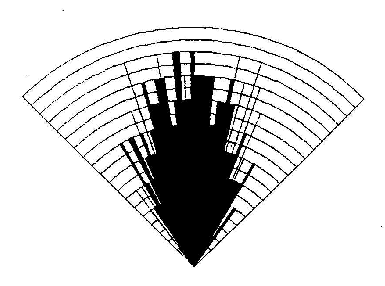
\includegraphics[scale=0.7]{ultra}
\caption{Spridning i ultraljudsavståndsmätarens mätningar. \autocite{spridning} }
\label{fig:ultra}
\end{figure}


 \section{Vinkelhastightessensor}
 Vinkelhastighetsmätare som ofta refereras till som gyroskop är en mekanisk sensor som kan detektera förändring av vinkel. Denna sortens sensorer kan användas för att räkna ut hur mycket roboten har roterat eller hur långt en sväng är gången. Vinkehastightessensor kan komplettera sensorerna som sitter på hjulen. Varför hjulens egna sensorer inte litas på 100\% är för att hjulen kan glida på underlaget eller slira. Detta skulle resultera i att roboten tror den har förflyttat sig när den stått still eller förflyttat sig för lite mot vad den får för information.
 
 \pagebreak
 
 \subsection{Fysikalisk princip}
 Vibrationsgyro sensorer känner av vinkelhastighet från Corioliskraften som verkar på ett vibrerande ojekt. Roboten kommer att roteras horisontellt - kring Z-axeln (se bild nedan), vilket leder till vertikal vibration inuti gyrot. Sedan beräknas potentiell skillnad mellan de vibrerande armar i gyrot och därmed uppskattas vinkelhastighet. [ref4] och [ref5]
 
\begin{figure}[H]
\centering
\includegraphics[scale=0.6]{gyro}
\caption{Vinkelhastighetssensor MLX90609 med axlar[ref?].}
\label{fig:gyro}
\end{figure}
 
 \subsection{Hur fungerar den för oss?}
 VHS innehåller en A/D-omvandlare, som konverterar data för att kommunicera med processorn via en SPI-bus.
 
 \subsection{Prestanda}
 Gyroskopet avläser 13-14 bitar, vilket beror på hur stor vinkelhastighet får vara. Roboten behöver egentligen inte att röra eller rotera sig snabbt. 

 \subsection{Störkänslighet}
 Vad kan göra att sensorn inte fungerar, vad får den att prestera sämre? Om chipet inte är helt vinkelrät kan det bli missvisande mätningar.
 
 
\section{Reflektionssensor}
Löst om sensorn

 \subsection{Fysikalisk princip}
 Beskriv hur sensorn fungerar
 
 \subsection{Hur fungerar den för oss?}
 Vad för info kommer vi få från sensorn
 
 \subsection{Prestanda}
 Hur bra är den på sin sak(enligt sig själv)

 \subsection{Störkänslighet}
 Vad kan göra att sensorn inte fungerar, vad får den att prestera sämre?
 
\section{RFID}
Löst om sensorn

 \subsection{Fysikalisk princip}
 Beskriv hur sensorn fungerar
 
 \subsection{Hur fungerar den för oss?}
 Vad för info kommer vi få från sensorn
 
 \subsection{Prestanda}
 Hur bra är den på sin sak(enligt sig själv)

 \subsection{Störkänslighet}
 Vad kan göra att sensorn inte fungerar, vad får den att prestera sämre?
 

\section{Resultat och slutsatser}
sammanfatta

\subsection{Diskussion}
Slutsats


\setcounter{secnumdepth}{0}
\pagebreak

\addcontentsline{toc}{section}{Referenser}

\printbibliography

%\section{Referenser}


%$^{[1]}$Vanheden, ISY:s datablad: %\url{https://docs.isy.liu.se/twiki/bin/view/VanHeden} \\[0.1in]

%[2] \url{http://www.acumo.se/generell-information-om-fotoceller-4}, 2015-03-04


%[figur~\ref{fig:sonar}] Principle of a sonar or radar distance measurement, Georg Wiora, \url{http://commons.wikimedia.org/wiki/File:Sonar_Principle_EN.svg}

%[figur~\ref{fig:ultra}] Vanheden om Ultraljud

%[4?] \url{http://www5.epsondevice.com/en/sensing_device/gyroportal/about.html}, 2015-03-05

%$^{[5?]}$Vanheden, ISY:s datablad:
%\url{https://docs.isy.liu.se/twiki/pub/VanHeden/DataSheets/MLX90609_datasheet.pdf}, 2015-03-05

\setcounter{secnumdepth}{2}
\end{flushleft}

\end{document}
